\documentclass[11pt]{book}

%--- PREREQUIS --- %
\usepackage{ifthen} % Options Si-Sinon pour les commandes latex

%Est-ce qu'on est sur un beamer ?
\newif\ifbeamer
\ifthenelse{\isundefined{\beamerbutton}}{\beamerfalse}{\beamertrue}

%--- GENERAL ---%
\usepackage{ucs}
\usepackage[utf8x]{inputenc} % Encodage du fichier
\usepackage[T1]{fontenc}  % Encodage des polices du document
\usepackage[english,francais]{babel} % Langages utilisés
\usepackage{lmodern} % Police pour rendre le texte sélectionable
\usepackage{pifont} % For access to weird symbols
\newcommand{\carriagereturn}{\Pisymbol{psy}{191}}

%\usepackage{xstring}

\ifbeamer
\else
\usepackage[top=2.5cm, bottom=2.5cm, left=2.5cm, right=2.5cm]{geometry} % Marges PDF
%\usepackage[top=2.5cm, bottom=2.5cm, left=2.5cm, right=3.5cm]{geometry} % Marges impression livre
\fi
\setlength{\parskip}{1ex plus .4ex minus .4ex}


%---BEAMER --- %
\ifbeamer
\usetheme{Darmstadt}
\useoutertheme[footline=institutetitle,subsection=true]{miniframes}
\setbeamertemplate{frametitle}[default][center] %titre centré
\addtobeamertemplate{footline}{\hfill\insertframenumber/\inserttotalframenumber\hspace{2em}\null}
%\usecolortheme{orchid}
%\usecolortheme{crane}

%Pour la transparence des pdf
\pdfpageattr {/Group << /S /Transparency /I true /CS /DeviceRGB>>} 
\fi

%--- STRUCTURES DONNEES ---%
\usepackage{enumerate} % Listes
\usepackage{array} % Tableaux
\usepackage{tabularx} % Tableaux modulables
\ifbeamer
\else
\usepackage[table]{xcolor} % Tableaux couleur
\fi
\usepackage{graphicx} % Figures
\usepackage[normalsize,up,bf,center]{caption2} % Meilleur distinction des figures
\renewcommand{\captionfont}{\bfseries \itshape}
\renewcommand{\captionlabeldelim}{~--}

% -- TABLEAUX ---- %
\usepackage{longtable} % Tableaux sur plusieurs pages
\usepackage{multicol} % Colonnes
\usepackage{multirow} % Lignes
\usepackage{rotating} % Écriture et figure verticales
\renewcommand{\arraystretch}{1.5} % Meilleur lisibilité des tableaux.

%--- MISE EN FORME & CARACTERES SPECIAUX ---%
\usepackage{amssymb} % Symboles
\usepackage{eurosym} % € symbol
\usepackage[autolanguage]{numprint} % 1000 => 1 000
\ifbeamer
\else
\usepackage[colorlinks=true,urlcolor=blue,pdfstartview=FitH,linkcolor=blue]{hyperref} % Liens
\fi
\usepackage{ulem} % Souligner, barrer, etc.
\usepackage{relsize} % Taille relative \smaller \bigger
\usepackage{color} % Couleur
\definecolor{darkred}{rgb}{0.72,0.16,0.11}
\definecolor{darkgreen}{rgb}{0.00,0.60,0.25}
\definecolor{darkblue}{rgb}{0.00,0.00,0.70}
\definecolor{brightblue}{rgb}{0.00,0.50,0.95}
\definecolor{darkpurple}{rgb}{0.58,0.07,0.49}
\definecolor{palegray}{gray}{0.80}
\definecolor{lightgray}{gray}{0.70}
\definecolor{pinkcomment}{rgb}{1,0,1}
\definecolor{keywordred}{rgb}{0.65,0.17,0.23}
\definecolor{pink}{rgb}{1,0.39,1}
\definecolor{violet}{rgb}{0.41,0.35,0.8}

\newcommand{\showcarriagereturn}{\color{green}\carriagereturn}
\newcommand{\showspace}{\color{green}\textvisiblespace}


%--- CODES SOURCES & CO ---%
\usepackage{verbatim} % Texte brut
\usepackage[french]{algorithm2e} % Algorithmes
\newenvironment{algo}[0]{\vrule~\vrule\itshape \begin{algorithm}[H] }{\normalfont\end{algorithm}}
\newcommand{\var}[1]{\textnormal{\texttt{#1}}}
\RestyleAlgo{plain}
\SetKwSwitch{Selon}{Cas}{Autre}{selon}{faire}{cas où}{autres cas}{fin}
\SetKwRepeat{Repeter}{r\'ep\'eter}{tant que}
\SetKwFor{uTq}{tant que}{faire}{} % Tant que sans fin (équivaut à uSi)
\SetKwFor{oTq}{}{}{fin} % Tant que déjà ouvert, donc sans balise de départ
\SetKwIF{oSi}{}{}{}{}{}{}{fin}
\SetKwIF{oFn}{}{}{fonction}{}{}{}{fin}
\SetKwFunction{KwFn}{Fn}



\usepackage{listings} % Codes sources
\usepackage{textcomp} % nécessaire pour upquote
\lstloadlanguages{[ANSI]C, sh, Python} % Listes de langages autorisés

% [style = sourceC] for the C codes
\lstdefinestyle{sourceC}{language=C, basicstyle=\small\color{black}\ttfamily, classoffset=0, keywordstyle=\color{blue}\bfseries, classoffset=1, morekeywords={NULL}, keywordstyle=\color{magenta}\bfseries, commentstyle=\color{brightblue}\itshape, stringstyle=\color{darkgreen}, showstringspaces=false, tabsize=3, framexleftmargin=2mm, frame=shadowbox, rulesepcolor=\color{lightgray}, breaklines=true, emph={main, printf, scanf, FILE, fopen, fscanf, fprintf, fclose, rand}, emphstyle=\color{darkblue}\bfseries,columns=fullflexible, flexiblecolumns=true, upquote=true, keepspaces=true}
% spaceflexible 

 
% Le langage C par défaut et le ANSI. On ne précise pas [ANSI] devant car cela pose problème si utilise le style dans un tableau 

% [style = python] for the python codes
\lstdefinestyle{python}{language=python, basicstyle=\small\color{black}\ttfamily, classoffset=0, keywordstyle=\color{blue}\bfseries, classoffset=1, morekeywords={NULL}, keywordstyle=\color{magenta}\bfseries, commentstyle=\color{brightblue}\itshape, stringstyle=\color{darkgreen}, showstringspaces=false, tabsize=3, framexleftmargin=2mm, frame=shadowbox, rulesepcolor=\color{lightgray}, breaklines=true, emph={main, printf, scanf, FILE, fopen, fscanf, fprintf, fclose, rand}, emphstyle=\color{darkblue}\bfseries,columns=fullflexible, flexiblecolumns=true, upquote=true, keepspaces=true}

% [style = msgTerminal] for shell codes
\lstdefinestyle{msgTerminal}{language=sh, basicstyle=\footnotesize\color{white}\ttfamily, keywordstyle=\color{white}, commentstyle=\color{white}\itshape, stringstyle=\color{white}, showstringspaces=false, framexleftmargin=3mm, xleftmargin=3mm, frame=none, tabsize=3, backgroundcolor=\color{darkgray}, rulecolor=\color{black}, breaklines=true,columns=fullflexible,upquote=true}

\lstdefinestyle{msgTerminalW}{language=sh, basicstyle=\small\color{black}\ttfamily, keywordstyle=\color{black}, commentstyle=\color{black}\itshape, stringstyle=\color{black}, showstringspaces=false, framexleftmargin=3mm, xleftmargin=3mm, frame=none, tabsize=3, backgroundcolor=\color{white}, rulecolor=\color{white}, breaklines=true,columns=fullflexible,upquote=true}

% [style = bash] for bash scripts
\lstdefinestyle{bash}{language=sh, basicstyle=\small\color{black}\ttfamily, classoffset=0, keywordstyle=\color{keywordred}\bfseries, morekeywords={mkdir, touch}, classoffset=1, morekeywords={$,$monNom,$RANDOM,$0,$1,$2,$3,$\#,$min,$max,$nomRep,$nom,$val,$elem}, keywordstyle=\color{magenta}\bfseries, commentstyle=\color{darkblue}\bfseries, stringstyle=\color{darkgreen}, showstringspaces=false, tabsize=3, framexleftmargin=2mm, frame=shadowbox, rulesepcolor=\color{lightgray}, breaklines=true, emph={main, printf, scanf, FILE, fopen, fscanf, fprintf, fclose}, emphstyle=\color{darkblue}\bfseries,columns=fullflexible,upquote=true}

%keywordstyle=\color{white}, commentstyle=\color{white}\itshape, stringstyle=\color{white}, showstringspaces=false, framexleftmargin=3mm, xleftmargin=3mm, frame=none, tabsize=3, backgroundcolor=\color{black}, rulecolor=\color{black}, breaklines=true,columns=fullflexible}

% [style = inlineSourceC] for C expression into text
\lstdefinestyle{inlineSourceC}{language=C, basicstyle=\footnotesize\color{black}\ttfamily, classoffset=0, keywordstyle=\color{blue}\bfseries, classoffset=1, morekeywords={NULL}, keywordstyle=\color{magenta}\bfseries, commentstyle=\color{brightblue}\itshape, stringstyle=\color{darkgreen}, showstringspaces=false, tabsize=3, breaklines=true, emph={main, printf, scanf, FILE, fopen, fscanf, fprintf, fclose, rand}, emphstyle=\color{darkblue}\bfseries,columns=fullflexible, keepspaces=true,upquote=true}
% Le langage C par défaut et le ANSI. On ne précise pas [ANSI] devant car cela pose problème si utilise le style dans un tableau (ne pas préciser frame=none non plus pour la même raison)

% [style = inlineTerminal] for shell expression into text
\lstdefinestyle{inlineTerminal}{language=sh, basicstyle=\footnotesize\color{black}\ttfamily\bfseries, keywordstyle=\color{black}, commentstyle=\color{black}\itshape, stringstyle=\color{black}\itshape, showstringspaces=false, tabsize=3, breaklines=true,upquote=true}
% Ne pas préciser frame=none pour laisser la possibilité d'utiliser le style dans un tableau

% [style = cadre] for printing an empty answer box (use framextopmargin=XXmm to set the height)
\lstdefinestyle{cadre}{language=[ANSI]C, basicstyle=\small\color{red}\ttfamily, showstringspaces=false, tabsize=3, framexleftmargin=2mm, frame=single, framerule=0.2mm, rulecolor=\color{black}, breaklines=true, columns=fullflexible, showlines=true,upquote=true}

% [style = sourceJava] for the Java codes
\lstdefinestyle{sourceJava}{language=Java, basicstyle=\small\color{black}\ttfamily, classoffset=0, keywordstyle=\color{darkgreen}\bfseries, commentstyle=\color{brightblue}\itshape, stringstyle=\color{darkgreen}, showstringspaces=false, tabsize=3, framexleftmargin=2mm, frame=shadowbox, rulesepcolor=\color{lightgray}, breaklines=true, emph={main, printf, FILE, fopen, fscanf, fprintf, fclose,new,return,this,super,null,break,continue,if,else,switch,case,default,do,while,for,break,new,return}, emphstyle=\color{darkred}\bfseries,columns=fullflexible,upquote=true}
% Le langage Java par défaut

% [style = sourceJava] for the Java codes
\lstdefinestyle{inlineSourceJava}{style=sourceJava, basicstyle=\normalsize\color{black}\ttfamily}
% Le langage Java par défaut


%--- CHEMINS DES DOSSIERS IMAGES---%
\graphicspath{{../../Commons/Images/} {./img/} {../../../../Commons/Images/}{../../../../../Commons/Images/}{../../../../../../Commons/Images/}{../../../Commons/Images/}}

% TODO : réintroduire une option pour se passer du paragraphe à la demande (ancienement none)

%FOR EACH pour parser différent arguments séparé par une virgule
%SPLIT pour séparer key=value
%Source : http://stackoverflow.com/questions/2402354/split-comma-separated-parameters-in-latex
%Plus bidouille A. Gademer (pour en déduire split)

\makeatletter

% Functional foreach construct 
% #1 - Function to call on each comma-separated item in #3
% #2 - Parameter to pass to function in #1 as first parameter
% #3 - Comma-separated list of items to pass as second parameter to function #1
\def\foreach#1#2#3{%
  \@test@foreach{#1}{#2}#3,\@end@token%
}

% Internal helper function - Eats one input
\def\@swallow#1{}

% Internal helper function - Checks the next character after #1 and #2 and 
% continues loop iteration if \@end@token is not found 
\def\@test@foreach#1#2{%
  \@ifnextchar\@end@token%
    {\@swallow}%
    {\@foreach{#1}{#2}}%
}

% Internal helper function - Calls #1{#2}{#3} and recurses
% The magic of splitting the third parameter occurs in the pattern matching of the \def
\def\@foreach#1#2#3,#4\@end@token{%
  #1{#2}{#3}%
  \@test@foreach{#1}{#2}#4\@end@token%
}

% Example-function used in foreach, which takes two params and builds hrefs
%\def\makehref#1#2{\href{#1/#2}{#2}}

% Using foreach by passing #1=function, #2=constant parameter, #3=comma-separated list
%\foreach{\makehref}{http://stackoverflow.com}{2409851,2408268}

% Will in effect do
%\href{http://stackoverflow.com/2409851}{2409851}\href{http://stackoverflow.com/2408268}{2408268}



% Functional Split construct 
% #1 - Function to call on each key=value items in #2
% #2 - key=value items to pass as parameter to function #1
\def\split#1#2{%
  \@test@split{#1}#2\@end@token%
}

% Internal helper function - Checks the next character after #1 and 
% continues loop iteration if \@end@token is not found 
\def\@test@split#1{%
  \@ifnextchar\@end@token%
    {\@swallow}%
    {\@split{#1}}%
}



% Internal helper function - Calls #1{#2}{#3}
% The magic of splitting the second parameter occurs in the pattern matching of the \def
\def\@split#1#2=#3\@end@token{%
  #1{#2}{#3}
}

\makeatother

% Example-function used in split, which takes two params
%\def\showbiz#1#2{Je vois #1 et #2.}

% Using foreach by passing #1=function, #2= key=value items
%\foreach{\showbiz}{key=value}

% Will in effect do
%Je vois key et value


% FIN FOR EACH et SPLIT




% PUPUCES !!!!! %

\newcommand{\pupuceC}[4]{\begin{center}\includegraphics[width=0.9cm]{#1} \color{#2}\\\textbf{#3}~\\\ifthenelse{\equal{#1}{quote}}{\itshape \og~#4~\fg}{#4}\end{center}}
\newcommand{\pupuceCN}[3]{\begin{center}\includegraphics[width=0.9cm]{#1} \color{#2}\\\textbf{#3}\vspace{-0.5cm}\end{center}}
 \newcommand{\pupuceLN}[4]{\includegraphics[height=0.6cm]{#1} \begin{minipage}{0.9\textwidth}  \color{#2}\textbf{#3}\end{minipage}}
 \newcommand{\pupuceL}[4]{\includegraphics[height=0.6cm]{#1} \begin{minipage}{0.9\textwidth}  \color{#2}\textbf{#3}~\ifthenelse{\equal{#1}{quote}}{\itshape \og~#4~\fg}{#4}\end{minipage}}
\newcommand{\pupuce}[5]{\ifthenelse{\equal{#1}{C}}{\pupuceC{#2}{#3}{#4}{#5}}{\ifthenelse{\equal{#1}{L}}{\pupuceL{#2}{#3}{#4}{#5}}{\ifthenelse{\equal{#1}{CN}}{\pupuceCN{#2}{#3}{#4}}{\ifthenelse{\equal{#1}{LN}}{\pupuceLN{#2}{#3}{#4}}{}}}}}

%--- DEFINITION DES ANNOTATIONS ---%

\newcommand{\error}[3][C]{\pupuce{#1}{error}{darkred}{#2}{#3}} % appel \error{TITRE}{TEXTE}

\newcommand{\warning}[3][C]{\pupuce{#1}{warning}{darkred}{#2}{#3}} % appel \warning{TITRE}{TEXTE}

\newcommand{\help}[3][C]{\pupuce{#1}{help}{brightblue}{#2}{#3}} % appel \help{TITRE}{TEXTE}

\newcommand{\info}[3][C]{\pupuce{#1}{information}{brightblue}{#2}{#3}} % appel \info{TITRE}{TEXTE}

\newcommand{\save}[3][C]{\pupuce{#1}{save}{darkgreen}{#2}{#3}} % appel \save{TITRE}{TEXTE}

\newcommand{\tips}[3][C]{\pupuce{#1}{tick}{darkgreen}{#2}{#3}} % appel \tips{TITRE}{TEXTE}

\newcommand{\ubuntu}[3][C]{\pupuce{#1}{UbuntuCoF}{orange}{#2}{#3}} % appel \ubuntu{TITRE}{TEXTE}

\newcommand{\quoted}[3][C]{\pupuce{#1}{quote}{darkpurple}{#2}{#3}} % appel \ubuntu{TITRE}{TEXTE}

\newcommand{\panicadvise}[3][C]{\pupuce{#1}{dont_panic}{brightblue}{#2}{#3}}

%\quoted{TITRE}{TEXTE}

\newcommand{\eureka}[0]{\includegraphics[height=36pt]{eureka}}
\newcommand{\dontpanic}[0]{\includegraphics[height=24pt]{dont_panic}}
\newcommand{\emosmile}[0]{\includegraphics[height=12pt]{emosmile}}




% CITATION DES SOURCES DES IMAGES
\newcommand{\bysa}[1]{\scriptsize{#1~\includegraphics[height=12pt]{cc_cc_30}\includegraphics[height=12pt]{cc_by_30}\includegraphics[height=12pt]{cc_sa_30}}}
\newcommand{\source}[1]{\begin{footnotesize} Source~:~#1 \end{footnotesize}}
\newcommand{\vsource}[1]{\begin{footnotesize} \color{gray} ~\begin{sideways}  \mbox{#1}\end{sideways} \end{footnotesize} }
\newcommand{\wikimedia}[1]{Wikimédia/#1}


%\begin{tableOfCommands}{nbcol}{disposition}{header}{légende}
% données du tableau
%\end{tableOfCommands}
\newenvironment{tableOfCommands}[4]{\begin{longtable}{#2}
\caption{#4}\tabularnewline
\hline   #3 \tabularnewline
\hline
\hline
\endfirsthead
\hline  #3  \tabularnewline
\hline
\hline 
\endhead
\multicolumn{#1}{c}{ (Suite page suivante)}\\
\endfoot
\hline
\endlastfoot}{\end{longtable}\medskip}

\newenvironment{tableOfCommandsNoCapt}[3]{\begin{longtable}{#2}
\hline   #3 \tabularnewline
\hline
\hline
\endfirsthead
\hline  #3  \tabularnewline
\hline
\hline 
\endhead
\multicolumn{#1}{c}{ (Suite page suivante)} \tabularnewline
\hline 
\endfoot
\hline
\endlastfoot}{\end{longtable}\medskip}

% % % % % % % % % % % % % % % % % % % % % % % % % % % % % % % % % % %
% Affichage de la division euclidienne et méthode de Horner !
% % % % % % % % % % % % % % % % % % % % % % % % % % % % % % % % % % %

\makeatletter
\newbox\nb@box
\newcount\nb@a
\newcount\nb@b
\newcount\iter@
\newcommand\division[2][2]{%
   \def\dividende@{#2}\def\base@{#1}\iter@\@ne\division@{#2}{#1}}
\newcommand\division@[2]{%
   \setbox\nb@box\hbox{\kern0.5em#1\kern0.5em}%
   \nb@a#1 \nb@b#1 \divide\nb@b#2
   \vtop{%
      \begingroup
         \multiply\nb@b#2 \advance\nb@a-\nb@b
         \hbox to\wd\nb@box{\hfil#1\hfil}%
         \vskip3pt\hrule height0pt width\wd\nb@box\vskip3.4pt
         \hbox to\wd\nb@box{\hfil\textbf{\color{red}\number\nb@a}\kern0.5em}%
         \expandafter\xdef\csname reste@\number\iter@\endcsname{\number\nb@a}%
      \endgroup}%
   \setbox\nb@box\hbox{8}\vrule height\ht\nb@box depth3.5ex
   \setbox\nb@box\hbox{\kern0.5em\ifnum#2>\nb@b #2\else\number\nb@b\fi\kern0.5em}%
   \vtop{%
      \hbox to\wd\nb@box{\kern0.5em#2\hfil}%
      \vskip3pt\hrule height0.4pt width\wd\nb@box\vskip3pt
      \hbox{%
         \csname @\ifnum\nb@b>\z@ first\else second\fi oftwo\endcsname
         {\advance\iter@\@ne\gdef\maxiter{\number\iter@}%
          \expandafter\division@\expandafter{\number\nb@b}{#2}}%
         {\kern0.5em\number\nb@b\xdef\maxiter{\number\iter@}}}}}

\newcommand\afficheresultat{$(\dividende@)_{10}=(\afficheresultat@\maxiter)_{\base@}$}
\newcommand\afficheresultat@[1]{%
   \csname reste@#1\endcsname
   \ifnum#1>\@ne
      \expandafter\expandafter\expandafter\afficheresultat@
   \else
      \expandafter\@gobble
   \fi{\number\numexpr#1-1}}
\makeatother

% % % % % % % % % % % % % % % % % % % % % % % % % % % % % % % % % % %
% Fin Affichage de la division euclidienne et méthode de Horner !
% % % % % % % % % % % % % % % % % % % % % % % % % % % % % % % % % % %



% Balises pour les questions & les exercices %
%\theoremstyle{definitionTP}
\usepackage[nocut]{thmbox}
\thmboxoptions{bodystyle=\noindent}
\newtheorem[L]{questionTheo}{\textbf{QUESTION}}
\newtheorem[L]{exerciceTheo}{\textbf{EXERCICE}}
\newtheorem[L]{correctionTheo}{\textbf{CORRECTION}}


\newenvironment{definitionTP}[1]{
\begin{tabular}{|m{1.3cm}m{0.8\textwidth}|}
\hline
\vspace{0.2cm}\includegraphics[width=1.3cm]{definition}&
\bfseries\underline{#1}~:}{
\tabularnewline
\hline
\end{tabular}
}




% L'environnement question est une encapsulation du théroème questionTheo
% On l'appelle de manière simple par \begin{question} ... \end{question}
% Si l'on veut marquer un type de question (Bonus, Défis), on peut écrire :
% \begin{question}[name=Défis} ... \end{question]
% ATTENTION, none est obligatoire si on a le paramètre optionnel
% Si l'on veut décrire le type de question, on peut écrire :
% \begin{question}[name=Défis,footnote=blah blah} ... \end{question]
% blah blah apparaitra en note de bas de page. :-)
%
% Attention à bien mettre la deuxième paire d'accollades (même vide) !
% Sinon vous perdez la première lettre de votre phrase
%
\makeatletter

%\newcommand{\setThmCut}[1][false]{\ifthenelse{\equal{#1}{false}}{\thmbox@cutfalse}{\thmbox@cuttrue}}

\newcommand{\parseExoArgs}[2]{
%Je vois #1 et #2.
\ifthenelse{\equal{#1}{cut}}{\ifthenelse{\equal{#2}{true}}{\thmbox@cuttrue}{}}{}% Découpage autorisé ?
\ifthenelse{\equal{#1}{name}}{\def\@name{#2}}{}%
\ifthenelse{\equal{#1}{label}}{\def\@label{#2}}{}%
\ifthenelse{\equal{#1}{footnote}}{%
\def\@footnote{\footnotemark}
\def\@footnoteTxt{#2}
}{}% Découpage autorisé ?
}

\newenvironment{exoreponse}[3]{
%A mettre au début de l'environnement.
\medskip%
\def\@name{none}%
\def\@footnote{}%
\def\@footnoteTxt{none}%
\def\@label{none}
\def\@theo{#2}%
\foreach{\split}{\parseExoArgs}{#1}% Parsing des options
\ifthenelse{\equal{\@name}{none}}{% Pas de noms (entre parenthèse)
\begin{\@theo}% 
}{%sinon
\begin{\@theo}[\@name\@footnote]%
}%
\ifthenelse{\not\equal{\@label}{none}}{%
\label{\@label}%
}{}%
\ifthenelse{\not\equal{#3}{none}}{% 
\includegraphics[height=20pt]{#3}%On affiche l'image associée
}{}%
}{% A mettre à la fin (attention, pas accès à #1 ni #2)
\end{\@theo}%
\ifthenelse{\not\equal{\@footnoteTxt}{none}}{\footnotetext{\@footnoteTxt}}{}%
}% Fin definition newenvirronment
\makeatother

\newenvironment{exercice}[1][]{
\begin{exoreponse}{#1}{exerciceTheo}{doit}%
}{%
\end{exoreponse}%
}% Fin definition newenvirronment

\newenvironment{question}[1][]{
\begin{exoreponse}{#1}{questionTheo}{question}%
}{%
\end{exoreponse}%
}% Fin definition newenvirronment

\newenvironment{correctionExo}[1][]{
\begin{exoreponse}{#1}{correctionTheo}{none}%
\color{red}\bfseries%
}{%
\end{exoreponse}%
}% Fin definition newenvirronment


%--- OBJECTIF TP EN AVANT PROPOS ---%
\newcommand{\abstractTP}[1]{\section*{Avant propos} \textit{#1}} % appel \abstractTP{TEXTE}

\newcommand{\difficulty}[1]{~\includegraphics[height=24pt]{difficult_#1}\protect\footnote{La difficulté estimé concerne le niveau et le temps de \underline{réflexion} nécessaire, pas la complexité algorithmique ou de programmation, qui sont à votre portée.}}




\usepackage{setspace}
\usepackage{appendix}

\title{Rapport de projet PAIR : Conception et implémentation d'un framework 
pour la création de réseaux multi-agents\\
PyMAS Framework}
\author{Timothée Duval \and Ebru Kizildas \and Franklin Raccah \\
\and Suivi par le Dr. Vincent Guyot}
\date\today

\begin{document}
\maketitle
\tableofcontents

\chapter*{Introduction}
\addcontentsline{toc}{chapter}{Introduction}
PyMAS \footnote{Python Multi-Agent System} est un Framework développé par 
notre groupe, cette année en language Python dans le but d’apporter une 
forme définie à un concept souvent mentionné mais rarement implémenté. Nous 
avons concu et développé un Système Multi-Agent modulaire, décentralisé et 
évolutif capable de s'exécuter sur une très grande partie du parc 
informatique mondial.

Cette caractéristique particulière est directement issue de notre choix 
d'utiliser le Python comme language de développement. Ce language objet 
interprété permet de faire fonctionner PyMAS sur les systèmes d'exploitation 
orientés "ordinateurs" (Windows, Unix, \dots \footnote{Développements et 
tests effectués sur GNU/Linux (Archlinux et Ubuntu), Windows 7, NetBSD 
et Mac OS X}) que sur un ordinateur embarqué ou un téléphone portable 
intelligent \footnote{Tests concluants sur iOS4 et Android 2.2.2} (pourvu des 
applications adéquates).

Cette portabilité permet de faire communiquer et coopérer de nombreux 
systèmes, et peut donc être implémenté aussi bien à l’échelle du grand 
public qu'à un niveau industriel.

Nous avons souhaité notre système modulaire, afin de ne pas limiter les
applications métiers dans les domaines que nous ne maîtrisons pas mais où 
l’informatique est présente et ou le paradigme multi-agent peut s'appliquer. 

Grâce à ce fonctionnement, il est possible pour un utilisateur de PyMAS 
d’intégrer ses propres modules développés en python ou dans un autre 
language, à condition que ces modules soient capables de fonctionner sur 
la machine hôte.

Ayant choisi de développer PyMAS avec une base de connexion pair à pair, 
c’est à dire communiquant de manière totalement décentralisée, nous avons 
dû nous pencher sur la sécurité de ce type de réseaux et intégrer de base, 
à notre framework des modules traitant la sécurité des communications.

Le livrable PyMAS consiste en un paquet Python permettant de lancer un agent 
sans fonction. Nous avons inclus dans ce paquet quelques modules nécessaires 
au fonctionnement minimal de PyMAS.

Ce framework est destiné à une utilisation par un autre projet de l'école 
travaillant sur de la domotique. Ce projet aura, à priori, lieu l'an 
prochain par des étudiants de l'association DTRE. \\
Un autre groupe d'étudiants a déjà choisi PyMAS pour un projet de 
robotique l'année prochaine.

\chapter{Analyse de l'existant}
Plusieurs projets connexes au notre sont déjà présents et disponibles sur 
internet et il nous fallait les observer, au moins rapidement de façon à ne
pas reproduire leurs éventuelles erreurs tout en nous en inspirant.

Nous recenserons ici trois projets présentant des aspect similaires au notre 
et expliciterons les différences avec PyMAS des points de vue techniques 
et conceptuels. Ces trois projets ont été choisis car ils représentent à 
eux trois les caractéristiques de la grande majorité des systèmes 
multi-agents actuels sur les problématiques que nous avons choisi de 
développer.

\section{Mango Automation}
Initialement prévu pour gérer une installation domotique, Mango Automation 
est constité d'un serveur, développé en Java se connectant à des agents qu'il
contrôle entièrement. Des plugins peuvent 
être écrits aisément via du JScript. Les tâches sont planifiées via des 
Timers et les seules interactions possibles entre agents sont de maître à 
esclave. Extrêmement aisé à prendre en main. 

Au delà du fait que la conception elle-même est centralisée, cette 
plate-forme est spécialisée en domotique.\\ 
De plus, nous recherchons, par notre projet une équivalence, au moins en 
conception, de tous les agents et non une intelligence possédée par 
un agent en particulier. Nous prendrons donc soin de bien répartir 
l'intelligence de groupe sur tous les agents.

\section{JACK}
De loin le plus poussé au niveau "recherche" de nos trois logiciels 
présentés. Plutôt performant, mais un peu lourd pour des besoins "habituels". 
Peu maniable sur des problématiques "physiques". Difficile à utiliser pour 
des utilisateurs lambda. JACK utilise son propre langage de scripting mais 
se base sur FIPA \footnote{Fundation for Intelligent Physical Agents. Le 
langage FIPA (FIPA ACL) ressemble à s'y méprendre à des structures de 
données LISP. \cite{o1998fipa}} pour les communications inter-agents.
Nous tenterons de simplifier au possible la mise en place de notre framework 
et d'utiliser des langages relativement populaires pour le scripting.

Utiliser FIPA pourrait, à terme être une bonne idée, ce qui permettrait 
d'interfacer PyMAS avec d'autres réseaux intelligents de recherche.

\section{Spyse}
Développé en Python, il s'agît également d’un framework de développement 
de systèmes multi-agents basés sur le modèle BDI.

Toutefois, la conception est pluri-centralisée en plateformes serveurs 
auxquelles les agents obéissent. Le développement de Spyse a été arrêté, 
fin 2009, et a donné suite à Pastiche, projet réunissant de nombreux 
aspects fonctionnels et étant par conséquent extrêmement lourd.

\section{Concepts similaires}
Au fur et à mesure de nos avancées, nous avons pu accéder à plusieurs 
concepts similaires développés dans le monde. Ces concepts nous ont sans 
conteste inspirés pour étendre les possibilités de PyMAS.

\subsection{Mother}
Mother est un ensemble de scripts développés par le hackerspace LVL1 
\footnote{\url{http://www.lvl1.org/}}. Cette 
IA globale se charge de monitorer différents capteurs, sites web, et de 
notifier les visiteurs du hackerspace. Elle est considéré comme un système 
domotique sans précédent par son évolutivité.

Il s'agît bien entendu d'un système centralisé, toutefois, nous avons voulu 
rendre accessible les même possibilités avec PyMAS. C'est donc en gardant à 
l'esprit les capacités d'adaptation de Mother que le développement en modules
s'est fait.

\subsection{Advogato}
Advogato est un réseau social dédié à l'OpenSource créé par Raph Levien ayant 
la particularité d'implémenter un système de confiance supposé résister à 
diverses attaques. \cite{levien1998attack} Toutefois, ce système repose 
essentiellement sur une activité humaine. 

Dans PyMAS, nous sommes fortement inspiré du système de mise en place de 
confiance d'advogato en le simplifiant. Nous étudierons ce système de 
confiance dans la suite de ce rapport.

\chapter{Architecture logicielle}
\section{Développement de modules indépendants}
Une des spécificités du Python reste la possibilité de développer aisément
en modules \cite{gcumodular}. Pour notre projet, nous avons choisi cette 
approche. Le projet est donc constitué de modules indépendants les uns 
des autres et séparés de manière pertinente (un module par action). 

Le développement modulaire présente plusieurs avantages, parmi lesquels la 
lisibilité du code et donc la facilité de troubleshooting reste le plus 
appréciable. On pourra également noter la possibilité de créer facilement 
une unicité de code globale dans le logiciel grâce à un prototype de 
module prédéfini. En cas d’erreur, on peut facilement isoler les 
modules problématiques pour mieux déboguer.

Dans le cadre de notre projet nous avons séparé nos modules en deux types : 
ceux bloquants et ceux non-bloquants. Les modules à action bloquante 
contiennent une ou plusieurs actions d’une durée non-négligeable et seront 
chacun démarrés dans un thread séparé tandis que les autres, considérés 
comme plus légers, seront exécutés séquentiellement dans la boucle 
principale de l'Agent.

Les modules apparaissent comme les parties "outils" de l'agent et 
permettent des intéractions effectives avec l'environnement. Chaque module 
a une forme standardisée précisant, pour chacun, les identifiants des 
beliefs pour lesquels il est utile, les mots de commande qu'il prend en 
compte et si son implémentation est bloquante ou non.

Chaque module correspond à un fichier Python déclarant au moins la variable
globale \verb?BLOCKING? pour définir si un module est bloquant ou non et 
optionnellement les variables globale : 

\begin{itemize}
\item \verb?USEFUL_FOR? : la liste des beliefs impactés par ce module
\item \verb?NECESSARY? : booléen définissant si le module s'exécute même 
avec une file d'attente de commandes vide
\item \verb?PRIORITY? : la priorité du module. Si celle-ci est négative, le 
module devient "necessary"
\item \verb?COMMAND_WORDS? : les mots de commande auxquels répond le module. 
Ce sont ces mots qui détermineront si le module est concerné par un commande 
ou non
\item \verb?COMMAND_RGX? : l'expression rationnelle dont la forme détermine 
les commandes auxquelles répond le module
\end{itemize}

Les méthodes suivantes sont à implémenter dans le module : 

\begin{itemize}
\item \verb?initialize()? : permet d’initialiser chaque module dès son 
chargement 
\item \verb?execute(cmd)? :  exécute la fonction principale du module 
concerné en l'appelant avec la commande reçue en argument
\item \verb?stop()? : (facultative) termine le module au déchargement de 
celui-ci
\end{itemize}

\begin{figure}
\begin{lstlisting}[style=python]
# Is this module blocking
BLOCKING = False
# Beliefs that are impacted by this module
USEFUL_FOR = ['nothing']
# Commands we can send to this module
COMMAND_WORDS = ['print', 'echo', 'say']
COMMAND_RGX = "^(print|echo|say)::.*?::"

def initialize(launcher):
    """Module initialization"""
    log.debug("Useless module initialization")

def execute(cmd_string):
    """Execute the command string"""
    cmd_list = cmd_string.split('::')
             
    print("Useless message : " + cmd_list[1])

\end{lstlisting}
\caption{Prototype d'un module}
\end{figure}

Il existe un autre aspect intéressant du développement modulaire : lorsque 
l'on utilise un module on ne se soucie pas de ce qui est à l'intérieur. 
Il suffit juste de connaître son effet. La probabilité d'erreur provenant 
d'une partie externe du programme est donc diminuée, on se concentre sur 
la modification du module en cours de développement.

\section{Communication entre modules via une file d'attente partagée}
Pour que chaque module puisse s'exécuter, nous avons opté pour l'utilisation
d'une fille d'attente partagée, représentant un bus de données logiciel. 
Cette file FIFO \footnote{First In First Out} contient toutes les commandes 
passées à chaque module. 

Il existe une file d'attente de commandes globale dont l'entrée est partagée 
indirectement par tous les modules. Chaque module a, à sa disposition propre, 
une file d'attente de commandes locale d'où sont tirées les commandes qu'il
reçoit.\\
Un thread de maintenance de la file de commandes est lancée de manière à 
recopier les éléments de la file globale dans toutes les files locales. En 
réalité, seules les références des commandes sont recopiées et non 
directement les objets, ne surchargeant pas la mémoire inutilement.

Certains modules peuvent ainsi générer de nouvelles commandes en vue que 
celles-ci soient utilisées par d'autres, créant ainsi une dépendance 
fonctionnelle et logique et non une dépendance entre classes. Par la méthode 
de la file d'attente partagée, l'indépendance des modules entre eux 
est d'autant plus marquée.

\begin{figure}[h]
  \begin{center}
    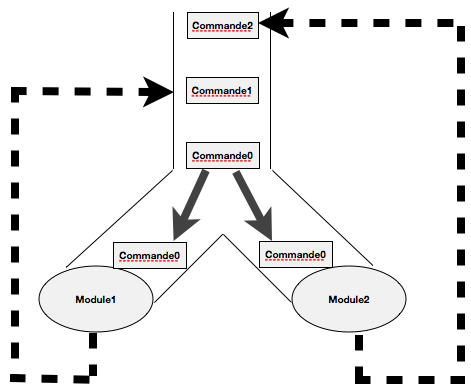
\includegraphics[width=12cm]{imgs/command_queue.png}
    \caption{File d'attente des commandes}
  \end{center}
\end{figure}

Les dépendances fonctionnelles entre module et une trop grande "explosion" 
des fonctionnalités restent toutefois à éviter pour ne pas ralentir le 
programme par des traitements et des itérations inutiles.

\section{Une configuration délimitée et nette}
Chaque agent dispose de sa configuration personnelle. Par défault, celle-ci 
se situe dans le répertoire \verb?~/.pymas?. \\
Pour plus d'ergonomie et de simplicité, cette configuration est en partie 
modifiable directement via la ligne de commande comme le montre le message 
d'aide ci-après.

\begin{figure}[ht]
\begin{lstlisting}[style=msgTerminal]
usage: pymas [-h] [-t] [-n NAME] [-m ADD_MODULE] 
[--disable-default-modules] [-D DIR] [-d | -i]

optional arguments:
  -h, --help            show this help message and exit
  -t, --no-write-conf   do not write the config file
  -n NAME, --name NAME  name of the agent
  -m ADD_MODULE, --add-module ADD_MODULE add a defined module to load
  --disable-default-modules Disable all default modules
  -D DIR, --directory DIR directory all pymas config, datas, and mods
  -d, --debug           make the debug in DEBUG mode
  -i, --info            make the debug in INFO mode
\end{lstlisting}
\caption{Message d'aide de PyMAS}
\end{figure}
\clearpage

Cette configuration est stockée dans un fichier JSON lisible humainement
via un simple éditeur de texte. Pour gérer cette configuration, nous 
utilisons un objet \verb?PersistorDirectory? lui-même contenant des objets 
\verb?Persistor?. Ces classes nous permettent de gérer aisément les accès à 
des fichier JSON du système via un dictionnaire \footnote{Objet "built-in" du
Python correspondant aux Map d'autres langages. Il faut y voir un ensemble 
d'association clef-valeur}

\begin{figure}[ht]
\begin{lstlisting}[style=python]
{
  "directory": "/home/mandarine/.pymas", 
  "modules": {
    "net_analyzer": {
      "severity": 4
    }, 
    "udp_listener": {
      "host": "", 
      "port": 7878
    }, 
    "udp_sender": {}, 
  }, 
  "name": "Smith"
}
\end{lstlisting}
\caption{Exemple de configuration}
\end{figure}

\section{Mise en forme de framework}
Ayant choisi de réaliser le projet sous forme de framework et prévoyant une
utilité très générique, la mise en modules est d'autant plus intéressante, 
permettant aussi bien pendant le développement (modules de base) que pendant 
l'utilisation (modules "métiers") de multiplier les points d'extensions.

Un framework est une forme de bibliothèque logicielle qui possède ses 
propres règles de développement, un certain nombre de fonctionnalités mères 
qui permettront à l'utilisateur d'intégrer celle dont il a besoin pour 
son projet. Il guide l'utilisateur dans son développement. De notre côté 
le développement de ce framework sous forme modulaire a facilité la 
division des tâches et accéléré la programmation de tâches diverses.

L’ensemble des modules et classes que nous avons fourni forment un noyau 
dont la fonctionnalité est de créer un réseau multi-agent capable d'agir de 
manière intelligente et de rester interconnecté de façon décentralisée.

Il est aisé de développer un système multi-agent à partir de PyMAS comme le 
montre notre script de test.

\begin{figure}[ht]
\begin{lstlisting}[style=python]
#!/usr/bin/env python
from pymas.config import Settings
from pymas.agents import Agent

def main():
    """Runs everything needed by the agent"""
    settings = Settings()
    agent = Agent(settings)
    agent.start()

    # The agent is executing
    try:
        agent.join()
    except KeyboardInterrupt:
        agent.stop()

if __name__ == '__main__':
    main()

\end{lstlisting}
\caption{Exemple de script d'exécution de PyMAS}
\end{figure}

\chapter{Intelligence de groupe}
\section{Modèle BDI}
Le modèle BDI \cite{bratman} constitue à la fois un modèle logiciel que nous 
avons utilisé et un modèle conceptuel très pratique pour appréhender 
l'Intelligence Artificielle par agent et donc, plus indirectement, 
l'Intelligence de groupe.

Ce modèle permet non seulement l'exécution séquentielle d'actions pour 
atteindre un ou plusieurs buts finaux simultanément, mais il permet aussi 
de donner des priorités à certaines \textit{intentions} ou certains 
\textit{désirs}.


\subsection{\textit{Beliefs, Desires, Intentions}}
Le modèle BDI est un modèle de développement informatique destiné à 
contrôler la façon dont un Agent se comporte \cite{haddadi1996belief}. Il 
est basé sur trois notions principales, les \textit{Beliefs}, les 
\textit{Desires} et les \textit{Intentions}.

\subsubsection{Les \textit{Beliefs}}
Les beliefs représentent les connaissances de l'agent sur lui-même et sur le 
monde qui l’entoure. Dans la pratique il s'agit par exemple d'une base de 
donnée contenant la liste des actions que l'agent est capable d'effectuer, 
de connaissances sur la température ou la luminosité ou encore de 
données sur les autres agents avec lesquels il est en communication.

Au sein d'un réseau multi-agents, certains beliefs sont partagés sur tout le
réseau. D'autres sont gardés et utilisés de manière interne à l'agent. 
L'acquisition d'une \textit{intention} unique (\textit{intention} ne devant 
être exécutée qu'une seule fois au sein de tout le réseau) passe par un 
\textit{belief}.

\subsubsection{Les \textit{Desires}}
Les \textit{desires} constituent les objectifs à long terme de l'agent et 
plus globalement du réseau. Ceux-ci peuvent être nombreux et même 
contradictoires. Il peut par exemple s'agir d'une action à effectuer de 
manière régulière ou d'une consigne à atteindre.

Dans un cadre multi-agent, les \textit{desires} sont tous partagés à travers 
le réseau. Les agents devront chacun observer les \textit{desires} et les 
\textit{belief}s à leur disposition afin de générer au mieux les 
\textit{intentions}\cite{astington1991developing}. 

\subsubsection{Les \textit{Intentions}}
Les \textit{intentions} sont les buts à très court terme. Il s'agît 
d'actions concrètes et finissable à relativement courte échéance. 
Les \textit{intentions} ne peuvent pas être contradictoires. Activées, elles 
se dirigent toutes vers un \textit{desire} particulier et se terminent 
possiblement avant la fin du \textit{desire}.

Les \textit{intentions} sont locales à chaque agent et peuvent être générées 
par groupes entiers pour chaque \textit{desire}. Certains agents, selon 
l'interconnection possédée avec leurs pairs, peuvent générer les 
intentions d'autres agents.\\
Ces intentions ne sont toutefois pas partagées pour autant et resteront 
locales à l'autre agent.

\subsection{BDI dans PyMAS}
Nous avons choisi d’implémenter ce modèle pour l'évidente raison qu'il est 
conçu pour la programmation de systèmes à agents 
\cite{jennings1993specification}. 

Dans notre framework les \textit{beliefs} sont représentés par des couples 
"clef/valeur" et sont stockés dans des objets persistants de façon à 
pouvoir en récupérer une partie au rechargement du logiciel. Les 
\textit{beliefs} sont, par défaut, partagés à travers tous les modules mais 
il est possible de masquer une partie de ceux-ci via des "vues".

Les \textit{desires} sont représentés par le chargement ou non d'un module 
dans l'agent. Certains modules comprennent en effet une consigne et 
surveillent celle-ci en même temps que leur état actuel afin de s'en 
rapprocher au mieux.

Les \textit{intentions} correspondent aux actions effectuées 
séquentiellement (ou parallèlement, dans le cas de modules bloquants) par 
le programme, qu'il s'agisse d'envoyer un message sur le réseau ou de 
contrôler un signal PWM \footnote{Pulse Width Modulation. Signal numérique 
modulé en largeur d'impulsion de façon à simuler un signal analogique} pour 
régler la vitesse d'un moteur.

\section{Logique floue}
La logique floue est un principe mathématique basé sur la théorie des 
ensembles flous. Elle est très utilisée, par exemple, en intelligence 
artificielle \cite{wang1994adaptive}.

Par opposition avec la logique booléenne, la logique floue considère qu'un 
état n'est pas forcément positif ou négatif, il peut se situer entre les 
deux comme l'illustre le graphe suivant.

\begin{figure}[h]
  \begin{center}
    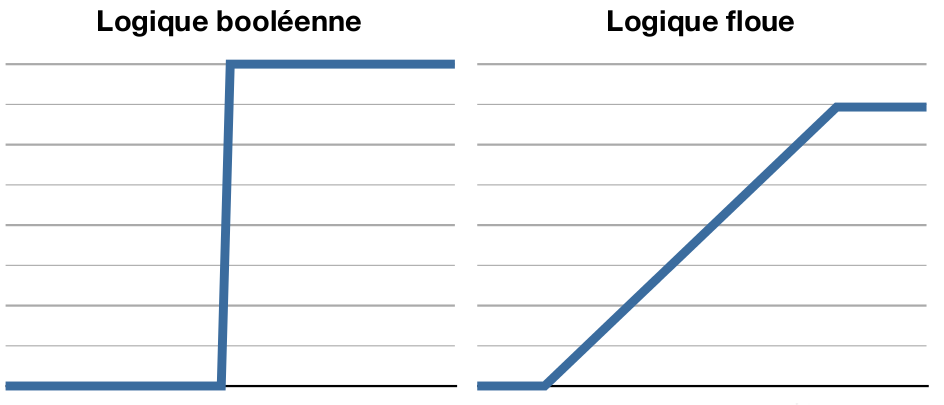
\includegraphics[width=13cm]{imgs/fuzzy_logic.png}
    \caption{Concepts de logiques}
  \end{center}
\end{figure}

Ceci permet de prendre des décisions plus justes, en ayant une indication 
quand à la valeur positive ou négative de la variable considérée. 
Evidemment la progression en logique floue n'est pas forcément linéaire 
comme représentée ci-dessus, en peut être de toute forme mathématique, ce 
qui permet de représenter toutes les situations qu'un agent pourrait 
rencontrer.

Cependant il vient un moment où une décision positive ou négative doit 
être prononcée. On utilise alors un seuil (18\% positif par exemple) pour 
prendre cette décision.

Dans PyMAS, cette logique est utilisée pour la sécurité des communications 
entre agents. La notion de confiance entre agents sera explicitée plus en 
détail dans la suite de ce rapport. La logique floue sert dans ce
contexte à déterminer si un message vient d’un agent auquel on peut faire 
confiance ou d’un inconnu. 

En plus de l’utilisation de cette logique mathématique, nous utilisons un 
seuil variable afin de s'adapter au mieux à la criticalité de l’action 
demandée par l'agent étranger. Une explication de l'utilisation du seuil 
variable est présente dans la partie "Sécurité" de ce rapport.

\section{Communication interne au réseau}
PyMAS, dans sa version minimale, contient plusieurs modules, parmi lesquels 
des modules de communication TCP et UDP. La raison semble logique : 
s'agissant d’un Framework Multi-Agent, il est nécessaire même dans une 
configuration minimaliste d’avoir des modules permettant la communication 
entre les Agents.

Nous avons développé un protocole de communication entre les Agents 
permettant à tous les individus de s'envoyer des commandes par le biais de 
tout réseau disponible. Les messages sont envoyés sous la forme de texte :
\verb?commande::argument_1,argument_1::signature_agent?

A la réception d'une commande réseau des modules d'analyse et de sécurité 
sont chargés de traiter l'information, de la comprendre et de vérifier 
si l'agent ayant envoyé le message est connu. Ce sont aussi ces modules qui 
vont lancer le traitement des commandes s'il est autorisé et maintenir la 
base de données d'agents connus. Les notions de sécurité liés à l'envoi 
de commandes entre agents seront expliquées plus en détail dans la suite 
de ce rapport.

Les agents sont capables de recevoir tout type de commande, qu'il s'agisse 
d'une simple création d'\textit{intention} d'allumer une diode ou 
d'ajouter un \textit{belief}. 

De manière à ce que le réseau évolue et se mette à jour automatiquement, 
il est possible de recevoir et de charger à la volée des modules depuis des
agents de confiance. Ces modules sont transmis via une suite de chaînes 
représentant le fichier en base64.

\chapter{Sécurité}
L'authentification, l'intégrité et la non-répudiation des messages est 
primordiale à nos yeux de façon à éviter une utilisation malveillante des 
réseaux multi-agents. Comment sécuriser un réseau dont les agents et la 
forme est inconnue ? Quelles méthodes actuelles de sécurité peuvent 
s'appliquer dans notre cas ?

\section{Signature numérique}
Les e-mails sont actuellement ce qui se rapproche le plus de la sécurisation 
que nous souhaitions incorporer à PyMAS. C'est donc tout naturellement que 
nous nous en sommes fortement inspiré.

\begin{figure}[ht]
  \begin{center}
    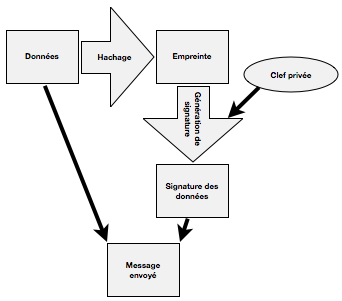
\includegraphics[height=9.5cm]{imgs/signature.png}
    \caption{Signature d'un message}
  \end{center}
\end{figure}


Le système de signature et de chiffrement de mails GPG nous a paru adapté 
à notre projet et c'est à ce titre que nous comptons, à terme, utiliser ses 
bindings Python (\verb?pygpg?) pour signer numériquement chaque messages. 
Utiliser GPG plutôt que d'entamer à la main cette procédure de signature 
numérique assurera pérennité et fiabilité.

La signature numérique la plus utilisée correspond à un système asymétrique 
et donc un système à deux clefs : une clef publique (que chaque agent se 
fait un plaisir de stocker dans ses beliefs et de diffuser à tous) et une 
clef privée qu'il garde pour lui et utilise pour signer. Cette clef 
privée n'est générée qu'une seule fois, au premier chargement du module 
correspondant. Il est primodial que cette clef reste inconnue du reste 
des agents et qu'elle ne soit pas diffusée. Cette clef est toutefois 
remplaçable, par d'autres moyens de génération, comme une carte sim ou une 
smartcart, sous réserve du développement d'un autre module de signature 
correspondant.

\begin{figure}[ht]
  \begin{center}
    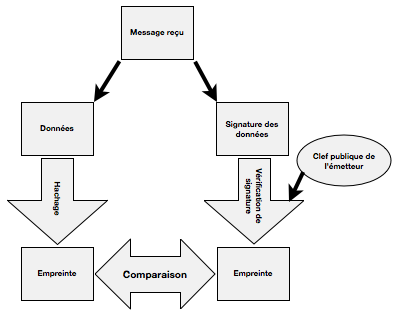
\includegraphics[height=9.5cm]{imgs/verification.png}
    \caption{Vérification de la signature d'un message}
  \end{center}
\end{figure}

Lorsqu'un message est reçu, selon sa teneur et la configuration de l'agent, 
la clef publique de l'agent qui a transmis le message sert à vérifier si 
le message provient bien de l'agent supposé émetteur. La signature est 
mise à part du message, à la fin de la transmission, de manière à ne pas 
interférer inutilement avec les arguments des commandes et à ne pas être 
traitée par les agents ne voulant pas s'encombrer d'une telle 
sécurité.

La signature numérique résoud donc les problèmes d'intégrité et de 
non-répudiation des données transmises. Toutefois, elle ne règle pas le 
problème bien plus conceptuel de la réaction à avoir face à une message 
venant d'un agent.

\section{Toile de confiance}
De façon totalement intégrée à GPG, une notion est apparue : celle de 
toile de confiance. Elle repose sur le fait que si un pair fait confiance 
à une signature numérique, et qu'une confiance en ce pair est considérée 
comme acquise, une confiance dans cette signature devrait être acceptable.

Comme précisé auparavant, l'acceptation et le maintien d'agents en tant 
"qu'amis" se fait via un algorithme utilisant la logique floue : la confiance
en un agent en particulier est symbolisée par une valeur entre -1 et 100 
(un \textit{belief}). Cette confiance varie à chaque intéraction (positive ou 
négative) avec cet agent.

\subsection{Création de relation}
\subsubsection{Métrique d'Advogato et Pagerank}
Ces deux métriques de confiance on déjà été déployées et mises à l'épreuve
\cite{ruder2004comparison}. C'est à ce titre que nous nous en sommes inspiré.

La métrique d'Advogato est une métrique de confiance supposée optimisée pour
la résistance à certaines attaques. Advogato se base sur un système à PKI
\footnote{Public Key Infrastructure} (semblable à celui de GPG). Il optimise 
la confiance en se basant sur les arrêtes du réseau et la distance par 
rapport au noeud concerné. \\
Toutefois cette métrique reste très limitée dans la mesure où les noeuds ne 
peuvent avoir que peu de niveaux de confiance (\textit{Apprentice}, 
\textit{Journeyer} et \textit{Master}) et les certifications de confiance se 
font humainement.

Le Pagerank est un algorithme créé par les fondateurs de Google. Il n'est 
pas du tout basé sur les arrêtes du réseau (cet algorithme étant créé pour 
le web, les distances sont toutes considérées à 1 saut) mais sur les 
relations entre pairs et le niveau de pertinence (de confiance) accordés 
les uns aux autres. Cet algorithme permet de diminuer fortement la 
probabilité d'une donnée arrivant sur un noeud reconnu comme relativement 
malveillant (un nombre réel détermine la confiance octroyée à un 
noeud). \\
Cependant, l'algorithme Pagerank peut être trompé \cite{wassner2012pagerank} 
via les attaques Sybil, entre autres.

Nous avons donc privilégié la création d'un algorithme hybride entre ces 
deux-ci. Notre métrique implémentera un niveau de confiance représenté par un
réel (comme dans le Pagerank) en étant basée à la fois sur les noeuds et sur 
les arrêtes. Les pairs de confiance devront valider les nouveaux venus et 
la confiance d'entrée attribuée devra dépendre de la distance réseau.

\subsubsection{Création d'une relation inter-agents dans PyMAS}
Lors de la connection d'un nouvel agent, un module d'analyse vérifie donc 
qu'il le connaît. Si ce n’est pas le cas, il stocke des renseignements sur 
cet agent avec un niveau de confiance nul puis envoie à tous ses agents
considérés comme "de confiance" \footnote{"De confiance" signifie que les 
agents en question ont un niveau de confiance supérieur à celui requis par 
l'action prévue. Dans ce cas précis, la valeur arbitraire de confiance a été 
fixée à 35. Les seuils de confiances sont définis par un module et sont 
stockés dans des \textit{beliefs}.} une demande d'identification de l'agent 
extérieur. Si l'un de ces "amis" a des informations, il répondra en joignant 
le taux de confiance qu'il porte au nouveau venu et des informations le 
concernant, dont sa clef publique. Celle-ci est vérifiée et l'agent est 
ensuite intégré avec un niveau de confiance calculé de manière arbitraire et 
naïve par la formule : 
\[ \sum \left ( \frac{\alpha_{i} \times t_{i}}{9500 + rand(100,300) \times 
K \times d_{i} } \right ) \]
Soit la somme de la confiance de chaque agent envers le nouveau venu 
($t_{i}$) pondérée par la confiance envers chacun de ces agents 
($\alpha_{i}$), la sévérité d'acceptation ($K$) et la distance séparant 
l'agent concerné de l'agent ami qui répond à la demande d'identification 
($d_{i}$). 

Il apparaît que, comme dans la métrique d'Advogato, plus la distance d'un 
point de vu "réseau" d'un agent est élevée, moins la confiance accordée 
peut-être grande. Privilégiant ainsi, une confiance dans les agents à 
peu de sauts réseaux. La mise en cause directe de cette distance est, en 
l'occurence relativement inutile, dans la mesure où la diminution de la 
confiance avec l'éloignement réseau se fait déjà ressentir sans. Elle est 
toutefois gardée de façon à ne pas oublier cette influence de la distance sur
la confiance accordée à un agent.
\begin{figure}[ht]
  \begin{center}
    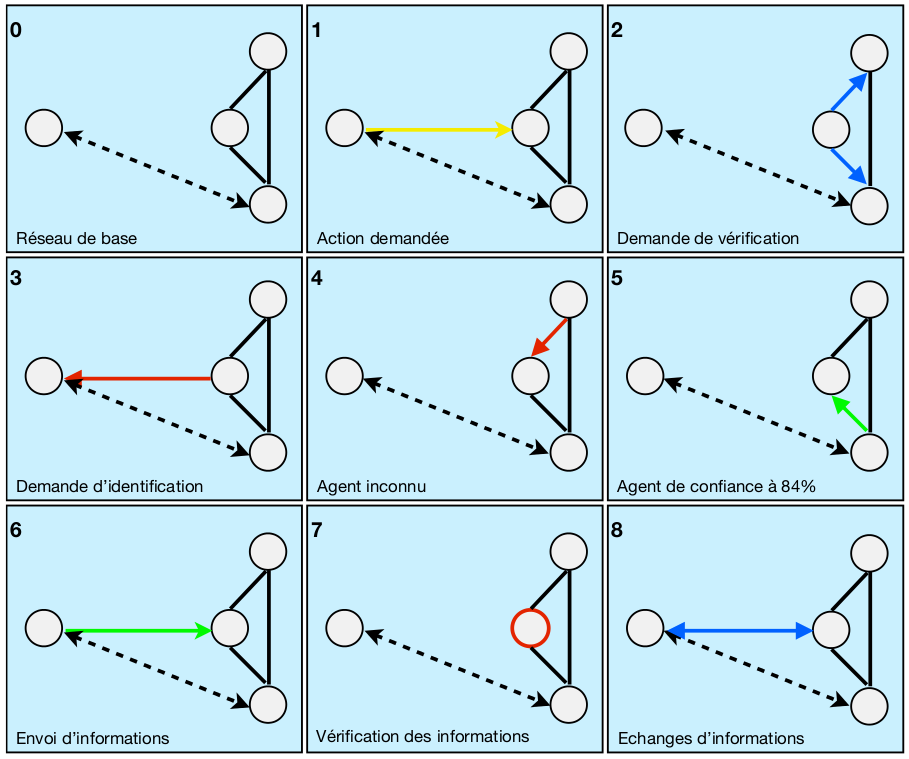
\includegraphics[height=13cm]{imgs/evolution.png}
    \caption{Création d'une relation depuis un nouvel agent}
  \end{center}
\end{figure}

\subsection{Construction de confiance}
Une fois la relation créée avec une confiance nulle, la relation évolue en 
confiance avec le temps, pouvant diminuer ou augmenter à chaque intéraction.
Dans PyMAS, chaque action demandée par un agent externe possède un seuil 
de confiance à atteindre avant d'être exécutée. Ce seuil a été fixé 
arbitrairement et est aisément modifiable. 

Pour la création de nouveaux \textit{beliefs} ou la mise à jour de 
\textit{beliefs} existant, le seuil demandé varie au cours du temps, selon le 
niveau de confiance de l'agent qui aura fait l'action précédemment. Par 
exemple, si un agent avec une confiance à 40 défini un \textit{belief} sur 
un autre agent, il faudra au minimum $80 \% \times 40 = 32$ pour redéfinir ce 
même \textit{belief}. Si personne n'a défini ce \textit{belief} auparavant, 
le seuil de confiance demandé est à $0$.

De la même façon, certaines actions de certains modules ont un seuil fixé "à 
la main" selon leur criticalité. Dans le cas d'un robot préparant du café, 
l'action de faire le café risquant de déclencher un problème physique et 
réel, son seuil de confiance minimum sera fixé à environ 75. \\
Le module gérant les cartes RFID étant très déterministe et relativement 
protégé bénéficiera d'un niveau de confiance à environ 80. Il n'est donc pas 
illogique de prévoir comme désir à notre réseau de préparer un café si un 
utilisateur passe sa carte RFID sur le lecteur.

\subsection{Perte de confiance}
Naturellement, le système de confiance deviendrait inutile s'il n'était pas 
possible de diminuer la confiance en un agent lorsque celui-ci fait preuve
d'un comportement anormal. Lorsqu'un agent répond mal à un \textit{belief}, 
dans la mesure où il est possible qu'il ne soit simplement pas encore mis à 
jour sur ce \textit{belief} particulier, il ne perd que $20 \%$ de la 
confiance qui lui était accordée jusque là.

Un module vérifie également continuellement les durées entre chaque. Pour 
toute tranche de 250 secondes où il n'y eu aucune intéractions entre deux 
agents, le niveau de confiance diminue de un point. 

\section{Vérifications continuelles}
Pour éviter un comportement malveillant ou chaotique, même après une 
validation parmi les "amis de confiance", certains modules sont prévus pour 
vérifier la confiance que l'agent peut apporter en chaque agent connecté. Ces 
modules fonctionnent de plusieurs façons.

\subsection{Vérification de beliefs}
L'agent envoie une demande de \textit{belief} non-critique dont il connaît 
déjà la valeur. Il pourra ainsi vérifier la validité des données renvoyées 
par l'agent étranger. \\
Un module se charge de contacter aléatoirement des agents amis avec certains 
\textit{beliefs} à vérifier.

Certains \textit{beliefs} concernent la durée de validité d'autres 
\textit{beliefs} et, si le module d'expiration des \textit{beliefs} est 
chargé, vérifier qu'un \textit{belief} expiré a bien la valeur 
\verb?expired? n'est pas spécialement à éviter, engendrant toujours une 
intéraction.

\subsection{Propagation de beliefs}
L'envoi d’un belief aléatoire sans utilité peut être pratique pour 
constater la propagation qui se fait sur le réseau. Elle permet également 
de vérifier qu’il n’y a pas altération des données. Pour cela, on demande 
à un agent (nommé A, dans cet exemple) la valeur de ce belief nous 
concernant, tout en lui répondant qu'il nous est inconnu. Celui-ci va 
alors demander à certains de ses agents amis et il est probable que la 
"question" se propage alors sur le réseau \footnote {Dans le choix de l'agent 
ami à contacter en premier, nous utilisons l'algorithme de Ford-Fulkerson, en 
utilisant la confiance comme valeur.}. Nous répondons bien la valeur du 
belief en question uniquement aux agents différents de A pour éviter les 
boucles de résolution.

\subsection{Inspiration du comportement humain}
De nombreuses autres façons de tester le réseau multi-agent créé sont 
possibles et s'inspirer du comportement humain est une bonne méthode de 
génération de tests. La génération d'un "brouhaha" nuit également au
réseau mais la légèreté du protocole l'empêchera relativement d’être 
utilisé pour une attaque par déni de service.

\chapter{Evolutions}
\section{Des modules supplémentaires}
Il ne s'agît pas tant d'une évolution que d'une application de PyMAS. Les 
modules "métier" peuvent toucher une grande variété de domaines. 
Nous souhaiterions toutefois augmenter les possibilités de base de PyMAS en 
lui ajoutant d'autres protocoles que le TCP et l'UDP dans les modules de base.

De la même façon, d'autres modules permettant d'interfacer plus simplement 
avec l'humain seraient à développer. Les modules de sécurité reste également
clairement à faire évoluer de façon à les rendre plus standards. \\
L'interprétation de commandes directement encodées en base64 serait 
potentiellement une bonne idée, même si cela nuira à la lisibilité du 
protocole par l'humain.

\section{Utilisation domotique}
Il s'agissait là de l'idée de base de notre projet et il est faisable de 
transmettre des messages à PyMAS via diverses interfaces. \\
Notons la présence d'un autre projet PAIR effectuant de la reconnaissance 
vocale pour générer des commandes PyMAS spécifiquement et d'un projet PSI 
contrôlant une machine à espresso contrôlable via le réseau.

Ces projets seront repris par l'association DTRE l'année prochaine en même 
temps qu'un projet de mini-robots communiquant de manière décentralisée via 
PyMAS.

\section{Utilisation communautaire}
Au même titre qu'Advogato, il est possible, via quelques nouveaux modules 
de mettre en place un réseau social simple via PyMAS. Chaque utilisateur 
peut publier du contenu reçu par les agents connectés ou qu'il souhaite 
contacter. \\
Implémenter un serveur web dans un module PyMAS est chose aisée et se baser 
sur des \textit{beliefs} pour contenir du contenu n'est absolument pas 
contraire à l'utilisation du framework. Toutefois, selon la taille des 
données et leur type (binaire ou non), il serait de meilleure conception de 
ne passer que des références au contenu en \textit{beliefs}.

\section{Chaotic Name System}
Chaotic Name System est un une idée de système DNS entièrement décentralisé
basé sur un système de confiance \cite{nicelab2012chaotic}. Il est possible 
de faire une implémentation du système DNS via PyMAS. Néanmoins, cela 
impliquerait que toute personne souhaitant annoncer un domaine sur le réseau 
devrait directement utiliser PyMAS. \\ 
Bien que cette évolution soit faisable techniquement, nous n'avons pas, pour 
le moment, l'intention de tenter d'appliquer PyMAS à ce cas.

\chapter{Problèmes rencontrés}
\section{Temps d'acceptation par le réseau}
A moins de corriger le seuil, l'acceptation par le réseau est longue et prend 
de (trop) nombreuses itérations. Deux manières de corriger cela sont 
d'augmenter les intéractions avec les nouveaux agents de façon à répartir la
prise de confiance du réseau pour un agent, ou de diminuer le seuil à 
partir duquel un agent est considéré "de confiance" pour effectuer chaque 
action. Cette seconde solution n'est que peu envisageable diminuant la 
sécurité du réseau.

\section{Attaques Sybil}
Les attaques Sybil peuvent être exécutées sur les réseaux pair à pair où est 
mise en place une relation de confiance. \cite{danezis2005sybil} 
Elle consiste en la génération de fausse confiance de la part d'un réseau 
virtuel de façon à montrer un large consensus. Ce réseau virtuel est 
représenté par une multitude de signatures différentes mais en réalité, 
issues de la même personnes \cite{shi2008smushing} et permet ainsi 
d'en prendre le contrôle en noyant la véritable information.

Pour éviter ce genre d'attaque relativement facile à réaliser, seuls 
les agents individuels connectés et leur niveau de confiance sont pris 
en compte. La métrique d'Advogato nous aura fortement servi d'inspiration 
dans ce cas.

\section{Petitesse de nos réseaux}
Au départ, nous étions attirés par l'idée d'une séparation des données sur 
le réseau. Toutefois, nous avons observé que la taille de notre réseau, même 
virtuel \footnote{Une cinquantaine d'agents lancés sur le même ordinateur} ne 
nous permettait pas d'utiliser ce genre de méthode. 

Nous nous étions en particulier penché sur la structure d'un arbre de Merkle 
pour une répartition des beliefs. Toutefois, pour un trop petit réseau, cette
structure n'a que peu de tolérance à la panne. Chaque agent garde donc une 
copie de tous les beliefs publics. Si un réseau utilisant PyMAS de grande 
envergure apparaît, il sera impossible de stocker tous les beliefs du réseau 
sur chaque agent. \\
Le développement d'un module de gestion des beliefs sous la forme d'un 
arbre de Merkle pourra être une des solutions envisageables et possibles.

\section{Abstraction nécessaire et visibilité}
Nous souhaitions voir notre projet réutilisé aussi bien au sein de l'ESIEA 
que dans le monde. Pour cela, il nous fallait éviter de fermer PyMAS à des 
applications auxquelles nous n'avions pas pensé. Nous avons donc dû faire 
preuve d'une grande abstraction durant le développement pour ne pas inclure
de modules métiers directement dans le coeur.

Nous avons également travaillé sur la visibilité du projet auprès de 
différents hackerspaces et communautés de façon à pouvoir mieux l'y
utiliser. \\
Le succès reçu aura dépassé nos attentes, recevant directement certaines 
offres d'entreprises et d'événements pour intégrer PyMAS à une solution 
existante ou plus simplement mener une intervention.

\chapter*{Conclusion}
\addcontentsline{toc}{chapter}{Conclusion}
Ce projet fut, pour nous un véritable pas en avant dans les domaines de 
l'intelligence artificielle et du réseau. 

C'est avec un grand plaisir que nous avons pu nous plonger plus avant dans 
divers concepts mathématiques, informatiques ou plus simplement logiciels à 
travers nos recherches et réalisation.

Nous aurons également pu rencontrer d'autres groupes de travail avec des 
idées de projets connexes et donc pouvions avancer ensemble en nous aidant 
mutuellement.

Nous sommes également ravis d'avoir contribué à un projet fortement orienté 
sur une problématique actuelle, à savoir : "L'Intelligence Artificielle au 
service de la sécurité". 

Enfin, nous tenons à remercier chaleureusement toutes les personnes nous 
ayant donné des pistes d'avancement et pour nous avoir encouragé à 
continuer ce projet.

\nocite*{}
\bibliographystyle{unsrt}
\bibliography{biblio}

\chapter{Annexes}
\section*{Diagrammes du projet}
\addcontentsline{toc}{section}{Diagrammes du projet}

\begin{figure}[ht]
  \begin{center}
    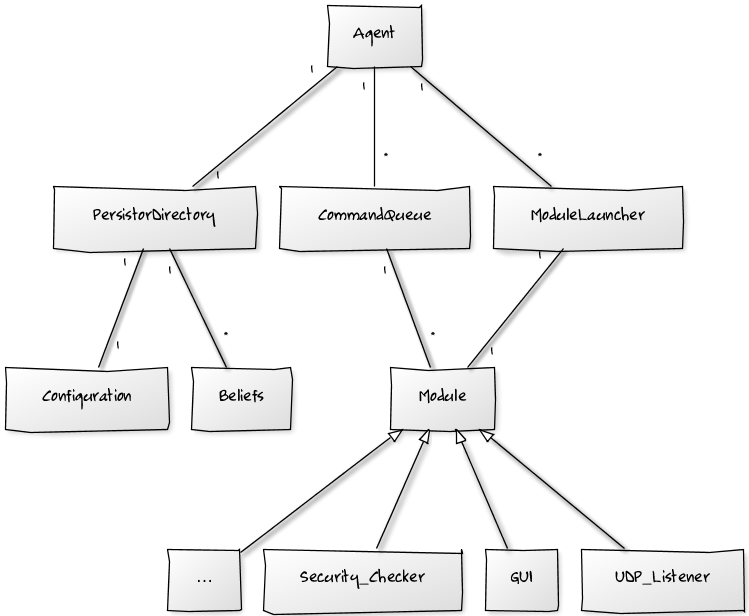
\includegraphics[width=13cm]{imgs/pymas_uml.png}
    \caption{Diagramme UML de classes simplifié}
  \end{center}
\end{figure}

\clearpage

\section*{Morceaux de codes choisis}
\addcontentsline{toc}{section}{Morceaux de codes choisis}
Le coeur de PyMAS et les modules systèmes sont directement accessibles sur
\url{https://github.com/DTRE/pymas}. Ceci représente le coeur du logiciel 
dans une version qui fonctionne sans être spécifiquement optimisée.\\
De nombreuses évolutions ont été faites depuis cette version du code et 
d'autres restent à venir dans les prochaines semaines.

\subsection*{persistor.py}
\addcontentsline{toc}{subsection}{Persistor.py}
\lstinputlisting[style=python]{codes/persistor.py}

\subsection*{config.py}
\addcontentsline{toc}{subsection}{Config.py}
\lstinputlisting[style=python]{codes/config.py}

\subsection*{modules/\_\_init\_\_.py}
\addcontentsline{toc}{subsection}{Modules/\_\_init\_\_.py}
\lstinputlisting[style=python]{codes/modules_init.py}

\subsection*{bdi.py}
\addcontentsline{toc}{subsection}{BDI.py}
\lstinputlisting[style=python]{codes/bdi.py}

\subsection*{modules/udp\_sender.py}
\addcontentsline{toc}{subsection}{Modules/UDP\_Sender.py}
\lstinputlisting[style=python]{codes/udp_sender.py}

\subsection*{modules/udp\_listener.py}
\addcontentsline{toc}{subsection}{Modules/UDP\_Listener.py}
\lstinputlisting[style=python]{codes/udp_listener.py}
\end{document}

